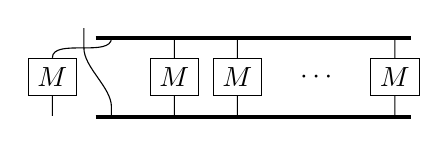
\begin{tikzpicture}
    \coordinate(O1)at(0,0);
    \coordinate(O2)at(0,-1);
    \draw[ultra thick]
        (O1)--++(4,0)
        (O2)--++(4,0)
    ;
    \draw
        (O1)++(1,0)--++(0,-.25)
        node[anchor=north, draw, rectangle](M1){$M$}
        (O2)++(1,0)--(M1.south)
        (O1)++(1.8,0)--++(0,-.25)
        node[anchor=north, draw, rectangle](M3){$M$}
        (O2)++(1.8,0)--(M3.south)
        (O1)++(3.8,0)--++(0,-.25)
        node[anchor=north, draw, rectangle](M2){$M$}
        (O2)++(3.8,0)--(M2.south)
        (O1)++(2.8,0)++(0,-.5)
        node[anchor=center]{$\cdots$}
        (O1)++(.2,0)
        % --++(0,-.125)
        .. controls ++(0,-.25) and ++(0,.25) .. ++(-.75,-.25)
        % --++(0,-.25)
        node[anchor=north, draw, rectangle](M0){$M$}
        (M0.south)--++(0,-.25)
        (O2)++(.2,0)--++(0,.125)
        .. controls ++(0,.25) and ++(0,-.25) .. ++(-.35,.75)
        --++(0,.25)
    ;
\end{tikzpicture}
